\begin{figure}[t]
    \centering
    \begin{subfigure}[b]{0.49\linewidth}
        \centering
        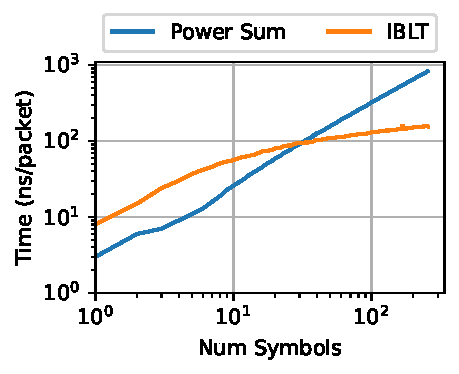
\includegraphics[width=\linewidth]{quack/figures/quack_encode.pdf}
        \caption{Encode time.}
        \label{fig:quack:iblt-computation:encode}
    \end{subfigure}
    \begin{subfigure}[b]{0.49\linewidth}
        \centering
        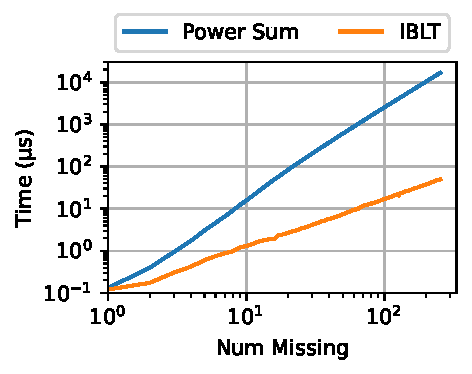
\includegraphics[width=\linewidth]{quack/figures/quack_decode.pdf}
        \caption{Decode time.}
        \label{fig:quack:iblt-computation:decode}
    \end{subfigure}
    \caption{IBLT vs. power sum quACK microbenchmarks. The number of trials is
     such that the cumulative time is at least $100$ ms. With rateless quACKs,
     the client can encode much larger numbers of symbols $t$ while the proxy
     decodes fewer symbols in the common case.
     % The logscale axes emphasize the overheads at smaller numbers.
     }
    \label{fig:quack:iblt-computation}
\end{figure}